% !TeX document-id = {0be8c18c-9430-4e9a-bdd9-12beadebfebc}
% !TeX TXS-program:bibliography = txs:///biber
\documentclass[11pt]{beamer}
\uselanguage{portuguese}
\languagepath{portuguese}
\deftranslation[to=portuguese]{Theorem}{Teorema}
\deftranslation[to=portuguese]{theorem}{teorema}
\deftranslation[to=portuguese]{Example}{Exemplo}
\deftranslation[to=portuguese]{example}{exemplo}
\deftranslation[to=portuguese]{Lemma}{Lema}
\deftranslation[to=portuguese]{lemma}{Lema}
\deftranslation[to=portuguese]{Corollary}{Corolário}
\deftranslation[to=portuguese]{corollary}{corolário}
%\deftranslation[to=portuguese]{and}{e}

\usepackage[brazilian]{babel}
\usepackage[utf8]{inputenc}
\usepackage[T1]{fontenc}
\usepackage{lmodern}
\usepackage{amsmath}
\usepackage{amssymb}
\usepackage{mathtools}
\usepackage{color}
\usepackage{pgfplots}
\usepackage{tikz}
\usepackage{subcaption}
%\usepackage{appendixnumberbeamer}

\newenvironment{transitionframe}{
	\setbeamercolor{background canvas}{bg=yellow}
	\begin{frame}}{
	\end{frame}
}
\usetheme{default}
\usefonttheme{structuresmallcapsserif}

%% I use a beige off white for my background
\definecolor{MyBackground}{RGB}{255,253,218}
\useinnertheme[shadow]{rounded}
\setbeamercolor{block title}{bg=MyBackground}
\setbeamercolor{block body}{bg=MyBackground}
\setbeamercolor{example title}{bg=MyBackground}
\setbeamercolor{example body}{bg=MyBackground}


\newcommand{\blue}[1]{\textcolor{blue}{#1}}
\newcommand{\red}[1]{\textcolor{red}{#1}}
\newcommand{\purple}[1]{\textcolor{purple}{#1}}
\newcommand{\gray}[1]{\textcolor{gray}{#1}}
\setbeamertemplate{navigation symbols}{}
%\setbeamertemplate{page number in head/foot}[appendixframenumber]

%\usepackage{graphics}
\usepackage{graphicx}

\definecolor{blue_emph}{RGB}{0,114,178}
\definecolor{red}{RGB}{213,94,0}
\definecolor{yellow}{RGB}{240,228,66}
\definecolor{green}{RGB}{0,158,115}
\definecolor{purple}{RGB}{204,121,167}
\definecolor{orange}{RGB}{230,159,0}
\definecolor{lightblue}{RGB}{86,180,233}

%\setbeamercolor{frametitle}{fg=blue}
%\setbeamercolor{title}{fg=blue}
\setbeamertemplate{footline}[frame number]
\setbeamertemplate{navigation symbols}{} 
\setbeamertemplate{itemize items}{-}
%\setbeamercolor{itemize item}{fg=blue}
%\setbeamercolor{itemize subitem}{fg=blue}
\setbeamertemplate{enumerate items}[default]
%\setbeamercolor{enumerate subitem}{fg=blue}
\setbeamercolor{button}{bg=MyBackground,fg=blue}
\usefonttheme{structuresmallcapsserif}

%\setbeamercolor{section in toc}{fg=blue}
%\setbeamercolor{subsection in toc}{fg=red}
\setbeamersize{text margin left=1em,text margin right=1em} 


\usepackage{appendixnumberbeamer}

\usepackage[
backend=biber,
style=authoryear,
natbib=true
]{biblatex}
\addbibresource{../bibliography.bib}

\newenvironment{wideitemize}{\itemize\addtolength{\itemsep}{10pt}}{\enditemize}
\newenvironment{wideenumerate}{\enumerate\addtolength{\itemsep}{10pt}}{\endenumerate}
\newenvironment{halfwideitemize}{\itemize\addtolength{\itemsep}{0.5em}}{\enditemize}
\newenvironment{halfwideenumerate}{\enumerate\addtolength{\itemsep}{0.5em}}{\endenumerate}


\author{Luis A. F. Alvarez}
\title{EAE1223: Econometria III}
\subtitle{Aula 6 - Modelos vetoriais autorregressivos}
%\logo{}
%\institute{}
\date{\today}
%\subject{}
%\setbeamercovered{transparent}

\begin{document}

\begin{frame}[plain]
	\maketitle
\end{frame}

\begin{frame}{Vetores aleatórios e matriz de variância-covariância}
\begin{halfwideitemize}
	\item Um vetor (coluna) aleatório $\boldsymbol{X}$, com valores em $\mathbb{R}^d$, é uma função com domínio no espaço de probabilidade $(\Omega,\Sigma,\mathbb{P})$ e contradomínio em $\mathbb{R}^d$.
\begin{itemize}
	\item Posto de outra forma, um vetor aleatório  $\boldsymbol{X}$ é um vetor cujas entradas $\boldsymbol{X}_j$, $j=1\ldots, d$, são variáveis aleatórias com valores reais.
\end{itemize}
\item Para um vetor aleatório $\boldsymbol{X}$, a matriz de variância-covariância, $\mathbb{V}[X]$, é definida como:

$$\mathbb{V}[\boldsymbol{X}]  = \mathbb{E}[\boldsymbol{X}\boldsymbol{X}'] - \mathbb{E}[\boldsymbol{X}]\mathbb{E}[\boldsymbol{X}']$$

\item Matriz de variância-covariância é $d \times d$, simétrica, positiva semidefinida, com entrada $(i,j)$ iguais a:

$$\mathbb{V}[\boldsymbol{X}]_{i,j}= \operatorname{cov}(\boldsymbol{X}_i,\boldsymbol{X}_j)\, .$$

\end{halfwideitemize}
\end{frame}

\begin{frame}{Matriz de covariância entre dois vetores aleatórios}
	\begin{itemize}
		\item Seja $\boldsymbol{X}$ um vetor aleatório em $\mathbb{R}^d$, e $\boldsymbol{Y}$ um vetor aleatório em $\mathbb{R}^p$, definimos a matriz de covariância entre $\boldsymbol{X}$ e $\boldsymbol{Y}$  como:
		
		$$\operatorname{cov}(\boldsymbol{X},\boldsymbol{Y}) = \mathbb{E}[\boldsymbol{X}\boldsymbol{Y}'] - \mathbb{E}[\boldsymbol{X}]\mathbb{E}[\boldsymbol{Y}'] \, .$$
		\item Matriz $d \times p$ em que a entrada $(i,j)$ é igual a:
		
		$$\operatorname{cov}(\boldsymbol{X},\boldsymbol{Y})_{i,j} = \operatorname{cov}(\boldsymbol{X}_i,\boldsymbol{Y}_j)$$
	\end{itemize}
\end{frame}

\begin{frame}{Processo vetorial fracamente estacionário}
\begin{itemize}
		\item Um processo estocástico vetorial é uma coleção de vetores aleatórios definidos em $\mathbb{R}^d$, indexados por um conjunto $\mathcal{I}$, isto é $\{\boldsymbol{X}_t: t \in \mathcal{I}\}$, onde cada $\boldsymbol{X}_t$ é vetor aleatório em $\mathbb{R}^d$.
		\begin{itemize}
			\item Cada entrada $j = 1\ldots d$ define um processo estocástico com valores reais $\{\boldsymbol{X}_{j,t}: t \in \mathcal{I}\}$ descrevendo a evolução da $j$-ésima entrada ao longo de $\mathcal{I}$.
		\end{itemize}
	\item Um processo estocástico vetorial $\{\boldsymbol{X}_t: t \in \mathcal{T}\}$ indexado no tempo $ \mathcal{T}$ é dito fracamente estacionário se:
	
	\begin{enumerate}
		\item$ \mathbb{E}[\boldsymbol{X}_t] = \boldsymbol{\mu}$ para todo $t \in \mathcal{T}$.
		\item $ \mathbb{V}[\boldsymbol{X}_t] = \Sigma_0$ para todo $t \in \mathcal{T}$, com $\operatorname{tr}(\Sigma_0) < \infty$.
		\item $\operatorname{cov}(\boldsymbol{X}_t,\boldsymbol{X}_{t-h}) = \Sigma_h$, para todo $t \in \mathcal{T}$, $h \in \mathcal{N}$.
	\end{enumerate}
	\item Extensão do conceito de série de tempo estacionária para o caso vetorial.
	\item Pedimos estabilidade das covariâncias contemporâneas e extemporâneas entre as entradas dos vetores.
	\item \textbf{Obs:} se processo é fracamente estacionária, cada uma das entradas $\{\boldsymbol{X}_{j,t}: t \in \mathcal{I}\}$ , $j =1,\ldots, d$, é fracamente estacionária.
\end{itemize}
\end{frame}

\begin{frame}{Ruído branco vetorial}
	\begin{itemize}
		\item Um processo estocástico vetorial  $\{\boldsymbol{X}_t: t \in \mathcal{T}\}$ com valores em $\mathbb{R}^d$ é dito um ruído branco vetorial se:
		
		\begin{itemize}
			\item $\mathbb{E}[\boldsymbol{X}_t] = \boldsymbol{0}_{d\times 1}$, para todo $t \in \mathcal{T}$.
		\item $ \mathbb{V}[\boldsymbol{X}_t] = \Sigma_0$ para todo $t \in \mathcal{T}$, com $\operatorname{tr}(\Sigma_0) < \infty$.
\item $\operatorname{cov}(\boldsymbol{X}_t,\boldsymbol{X}_{l}) = \boldsymbol{0}_{d\times d}$, para todo $t \neq l$.
		\end{itemize}
		\item No ruído branco vetorial, permitimos associação contemporânea entre as entradas do vetor, mas não há nem autodependência nem dependência cruzada entre as entradas no tempo.
	\end{itemize}
\end{frame}

\begin{frame}{Ruído branco vetorial Gaussiano}
$$\begin{pmatrix}
	{\epsilon_{1,t}} \\
		{\epsilon_{2,t}}
\end{pmatrix} \overset{\text{iid}}{\sim} \mathcal{N}\left(\begin{pmatrix}
0 \\
 0
\end{pmatrix} , \begin{pmatrix}
1 & 1 \\
1 & 2
\end{pmatrix}\right)$$
\begin{figure}
	\centering
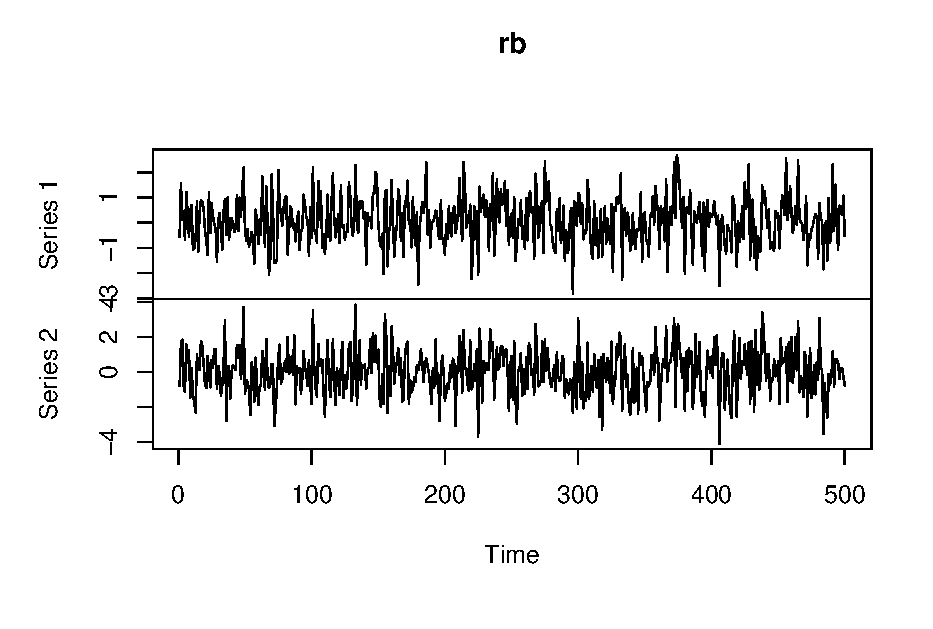
\includegraphics[scale=0.7]{graficos/rb_multi.pdf}
\end{figure}

\end{frame}

\begin{frame}{Modelos vetoriais autorregressivos}
	\begin{itemize}
		\item Considere $d$ séries de tempo $\{X_{j,t}: t \in \mathbb{Z}\}$, $j=1,\ldots, d$.
		\item Dizemos que estas séries definem um processo vetorial autorregressivo de ordem $p$, ou VAR(p), se, para todo $j=1,\ldots, d$ e $t\in \mathbb{Z}$:
	\end{itemize}
	\begin{equation*}
		\begin{aligned}
			X_{{\color{blue}j},t} &= a_{{\color{blue}j},0}  +\sum_{l=1}^p a_{{\color{blue}j},{\color{orange}1},l} X_{{\color{orange}1},t-l} + \sum_{l=1}^p a_{{\color{blue}j},{\color{orange}2},l} X_{{\color{orange}2},t-l}   +\ldots + \sum_{l=1}^p a_{{\color{blue}j},{\color{orange}d},l} X_{{\color{orange}d},t-l}  + \epsilon_{{\color{blue}j},t} \\
			&= a_{{\color{blue}j},0}  +{\color{orange}\sum_{k=1}^{d}}\sum_{l=1}^p a_{{\color{blue}j},{\color{orange}k},l} X_{{\color{orange}k},t-l} + \epsilon_{{\color{blue}j},t} \, ,
		\end{aligned}
	\end{equation*}
	onde $\boldsymbol{\epsilon}_t = (\epsilon_{1,j,t},\epsilon_{2,j,t},\ldots, \epsilon_{d,j,t})'$ é um ruído branco vetorial.
	\begin{itemize}
		\item No VAR(p), assim como no AR(p), evolução em cada uma das $d$ variáveis depende do que ocorreu nela mesma nos últimos $p$ períodos.
		\item Mas além disso, trajetória depende do que ocorreu nos últimos $p$ períodos {\color{orange}nas demais variáveis}.
		\item Série depende também de uma inovação $\epsilon_{j,t}$, imprevisível com base no passado, mas que pode estar contemporaneamente associada às demais inovações nas outras equações (choques comuns).
	\end{itemize}
\end{frame}

\begin{frame}{VAR(p) em notação vetorial}
	\begin{itemize}
		\item Um VAR(p) pode ser escrito, compactamente, em notação vetorial.
		\item De fato, definindo $\boldsymbol{X}_t = (X_{1,t},X_{2,t},\ldots, X_{d,t})'$, podemos escrever o sistema como
		
		\begin{equation*}
			\boldsymbol{X}_t = \boldsymbol{a}_0 + \boldsymbol{A}_1 \boldsymbol{X}_{t-1} + \boldsymbol{A}_2 \boldsymbol{X}_{t-2} + \ldots + \boldsymbol{A}_p \boldsymbol{X}_{t-p} + \boldsymbol{\epsilon}_t \, ,
		\end{equation*}
		onde
		$$\boldsymbol{a}_0 = \begin{bmatrix}
			a_{1,0} \\
			a_{2,0} \\
			\vdots \\
			a_{d,0}
		\end{bmatrix} \quad \quad \boldsymbol{A}_l = \begin{bmatrix}
			a_{1,1,l} & 	a_{1,2,l} & \ldots &	a_{1,d,l} \\
			a_{2,1,l} &  	a_{2,2,l}  &  \ldots & a_{2,d,l} \\
			\vdots & \vdots  & \ldots & \vdots  \\
			a_{d,1,l} & a_{d,2,l} & \ldots & a_{d,d,l}
		\end{bmatrix}$$ 
	\end{itemize}
\end{frame}
\begin{frame}{VAR(p) estacionário}
	\begin{itemize}
		\item Um VAR(p) é dito estacionário se o processo vetorial resultante é estacionário.
		\item Condição para estacionariedade do VAR(p) é que:
		
		$$ |z| \leq 1 \implies \operatorname{det}(\mathbb{I}_{d\times d} - \boldsymbol{A}_1 z - \boldsymbol{A}_2 z^2 \ldots -  \boldsymbol{A}_p z^p ) \neq 0$$
		\item Todas as raízes do polinômio $\phi(z) = \operatorname{det}(\mathbb{I}_{d\times d} - \boldsymbol{A}_1 z - \boldsymbol{A}_2 z^2 \ldots -  \boldsymbol{A}_p z^p )$ devem se encontrar fora do círculo unitário.
		\item Nesta aula, focaremos na estimação de VAR(p) estacionários.
		\begin{itemize}
			\item Portanto, cada uma das séries deverá estar devidamente estacionarizada. 
		\end{itemize}
	\end{itemize}
\end{frame}
\begin{frame}{Estimação do VAR(p)}
	\begin{itemize}
		\item 	Dado um painel com observações de $d$ séries durante $T$ períodos, $\{\boldsymbol{X}_{j,t}\}_{t=1}^T$, como estimar os parâmetros de um VAR(p)?
		\item Maneira mais simples é estimar os parâmetros através de MQO, {\color{blue}equação a equação}.
		\item Isto é, estimamos os parâmetros da $j$-ésima equação resolvendo:
		
		$$\min_{b_{0,j}, \{b_{j,k,l}\}_{k,l}} \sum_{t=p+1}^T\left(\boldsymbol{X}_{j,t} - b_{0,j} - \sum_{k=1}^d \sum_{l=1}^p b_{j,k,l}X_{j,t-l}\right)^2$$
		\item Para cada equação, rodamos uma regressão com $T$ observações e $p\times d +1$ parâmetros.
	\end{itemize}

\end{frame}

\begin{frame}{SUR}
	\begin{itemize}
		\item A estimação dos parâmetros de um VAR por MQO, equação a equação, é potencialmente ineficiente.
					\item Isso se deve ao fato de que os choques em uma equação $j$, por serem (potencialmente) contemporaneamente correlacionados com os choques das demais equações, podem conter informação relevante para estimar os parâmetros de outras equações
		\begin{itemize}
		\item Erro em uma equação é informativo sobre a outra equação.
		\end{itemize}
		\item Seja $\hat \Sigma_0$ um estimador preliminar de $\mathbb{V}(\epsilon_t)$.
		\begin{itemize}
			\item Por exemplo, estimador da variância-covariância com base nos resíduos do estimador de MQO equação a equação.
		\end{itemize}
		\item O estimador de \textit{seemingly unrelated regression} (SUR) dos parâmetros de um VAR propõe-se a estimar os parâmetros do sistema {\color{blue}conjuntamente}, minimizando:
	\end{itemize}		$$\min_{\boldsymbol{b}_0, \boldsymbol{B}_1,\ldots \boldsymbol{B}_p} \sum_{t=p+1}^T \left(\boldsymbol{X}_t - \boldsymbol{b}_0 -  \sum_{l=1}^p\boldsymbol{B}_l \boldsymbol{X}_{t-l}\right)' \hat \Sigma^{-1} \left(\boldsymbol{X}_t - \boldsymbol{b}_0 -  \sum_{l=1}^p\boldsymbol{B}_l \boldsymbol{X}_{t-l}\right)$$
\end{frame}
\begin{frame}{Máxima verossimilhança condicional}
\begin{itemize}
	\item Sob a hipótese auxiliar:
	
	$$\boldsymbol{\epsilon}_t \overset{iid}{\sim} N(\boldsymbol{0}_{d\times 1}, \Sigma_0)$$
	podemos calcular a verossimilhança de $\boldsymbol{X}_{t+p+1},\ldots \boldsymbol{X}_{T}$, condicional a $\boldsymbol{X}_1,\ldots, \boldsymbol{X}_p$.
	\item Estimador de máxima verossimilhança condicional estima {\color{blue}simultaneamente} $\boldsymbol{a}_0$, os $\boldsymbol{A}_l$  e $\Sigma_0$.
\end{itemize}
\end{frame}
\begin{frame}{Relação entre os métodos de estimação}
\begin{itemize}
	\item Se o espaço de parâmetros é irrestrito, no sentido de que os parâmetros $\boldsymbol{a}_0$ e os $\boldsymbol{A}_l$ podem tomar qualquer valor real, os estimadores de MQO equação a equação, SUR, e máxima verossimilhança condicional são {\color{blue}numericamente iguais}.
	\item Se impomos restrições nos parâmetros $\boldsymbol{a}_0$ e os $\boldsymbol{A}_l$, estimador de MQO equação a equação é consistente, embora SUR e máxima verossimilhança condicional sejam mais eficientes.
	\item Se, além disso, impomos restrições na matriz ${\Sigma}_0$, os três estimadores são consistentes, mas máxima verossimilhança condicional é o mais eficiente.
\end{itemize}
\end{frame}
\appendix
\begin{frame}{Referências}
	\printbibliography
\end{frame}
\end{document}

